\documentclass{beamer}

\usepackage{comment}
\usepackage{color}

\title{Unstructured Grids}
\author{Glenn Hammond}
\date{\today}

\begin{document}
  
\frame{\titlepage}


\subsection{Type of Unstructured Grids}

\begin{frame}[fragile]\frametitle{Types of Unstructured  Grids}

\begin{itemize}
  \item UNSTRUCTURED
  \begin{itemize}
     \item PFLOTRAN naming convention: \textit{Implicit} Unstructured (.ugi)
     \item Finite element approach (cells and vertices)
     \item Cell are defined by a list of vertices.
     \item Vertices are define by coordinates.
     \item \textbf{Cell and connectivity information is calculated internally (e.g. centroid, volume, area, distance).}
   \end{itemize}
  \item UNSTRUCTURED\_EXPLICIT
  \begin{itemize}
     \item PFLOTRAN naming convention: \textit{Explicit} Unstructured (.uge)
    \item Cells are defined with an ID, coordinate, and volume.
    \item Connections are defined with two grid cell IDs, a coordinate for the intersection with the face and an area.
    \item \textbf{Cell and connectivity information is explicitly defined through input.}
  \end{itemize}
\end{itemize}

\end{frame}

\begin{frame}[fragile]\frametitle{UNSTRUCTURED (Finite Element)}
\vspace{0.2in}
\centering
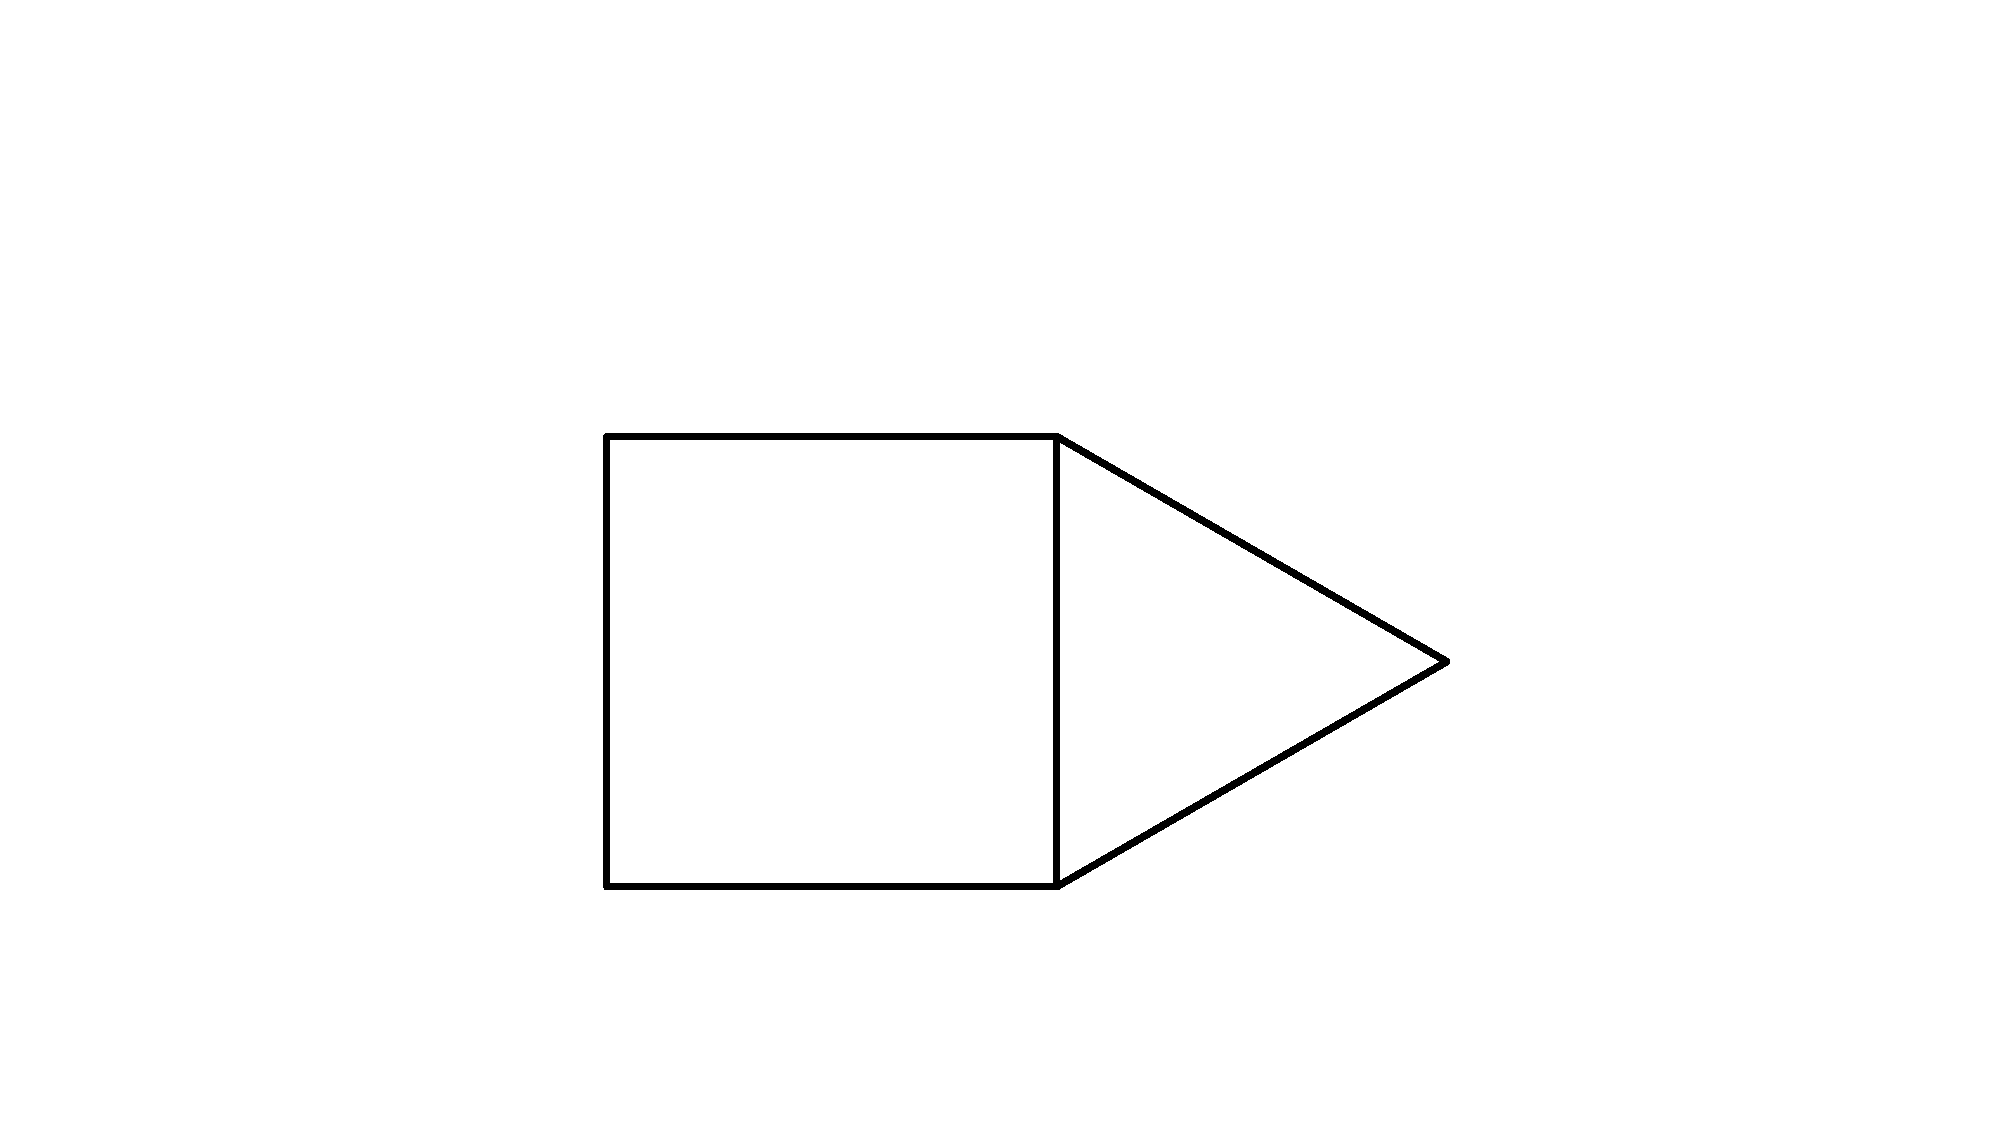
\includegraphics[width=1\linewidth]{./fe_geom}
\end{frame}

\begin{frame}[fragile]\frametitle{UNSTRUCTURED (Finite Element)}
\vspace{0.2in}
\centering
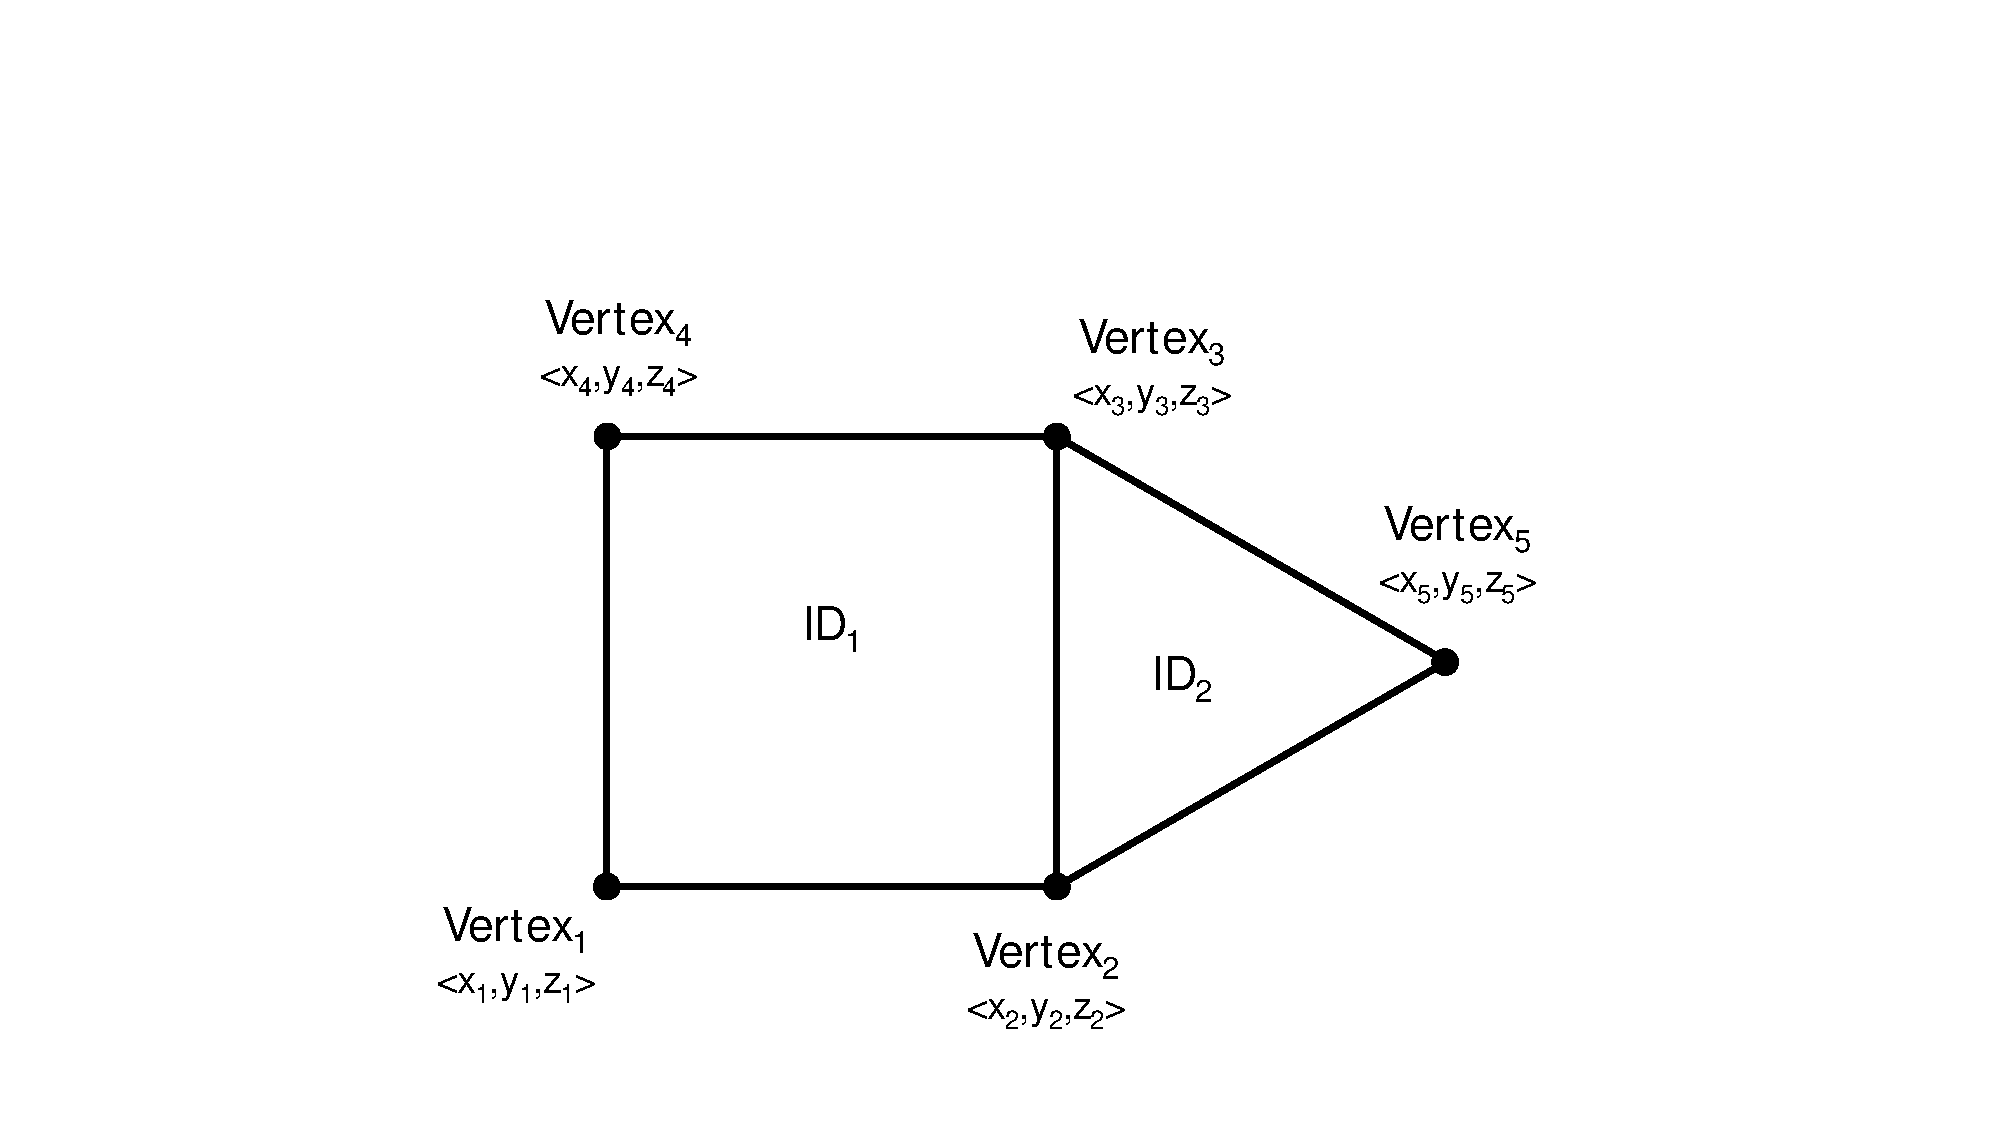
\includegraphics[width=1\linewidth]{./fe_raw}
\end{frame}

\begin{frame}[fragile]\frametitle{UNSTRUCTURED (Finite Element + Connectivity)}
Centroids, distances, areas and volumes are calculated internally.
\vspace{0.2in}
\centering
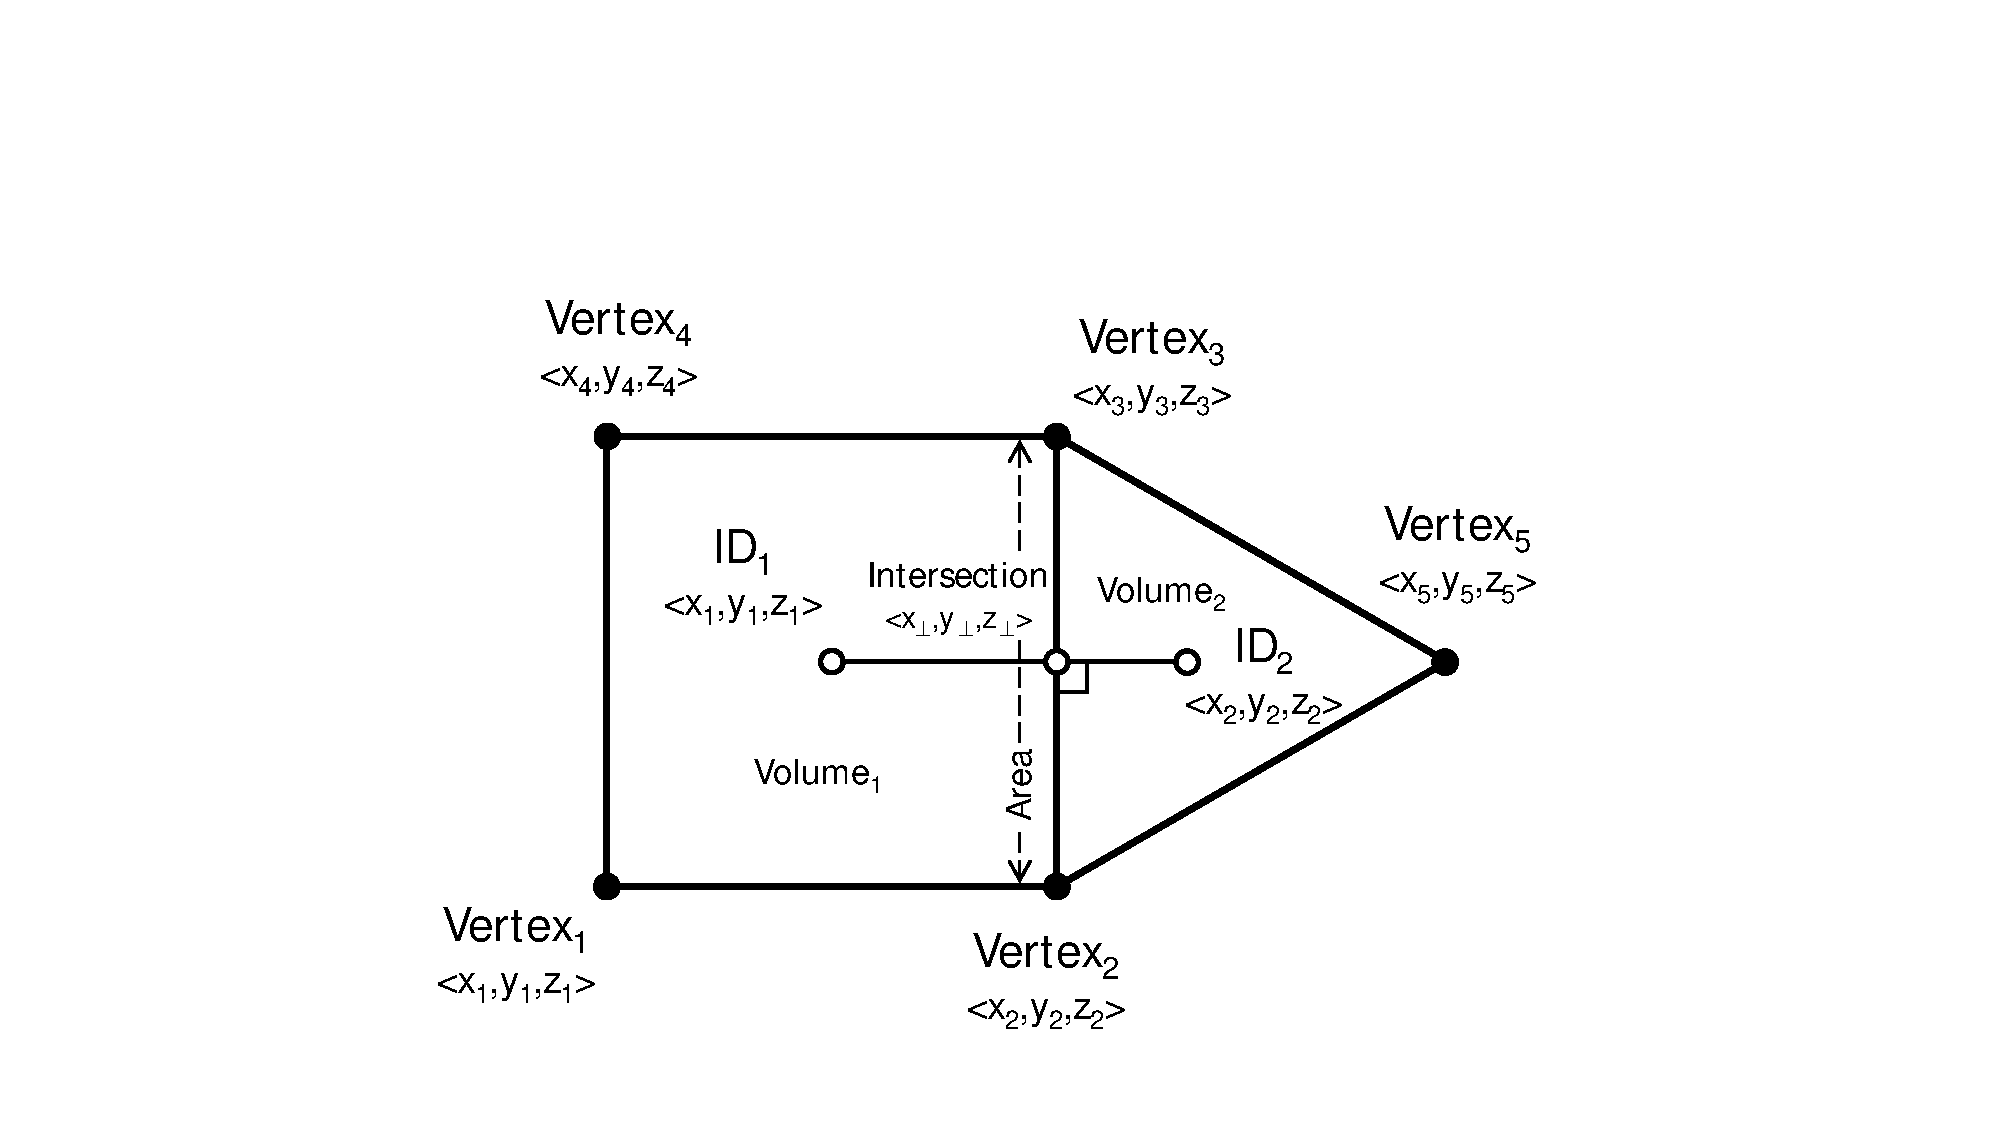
\includegraphics[width=1\linewidth]{./fe_all}
\end{frame}

\begin{frame}[fragile]\frametitle{UNSTRUCTURED (Connectivity)}
\vspace{0.2in}
\centering
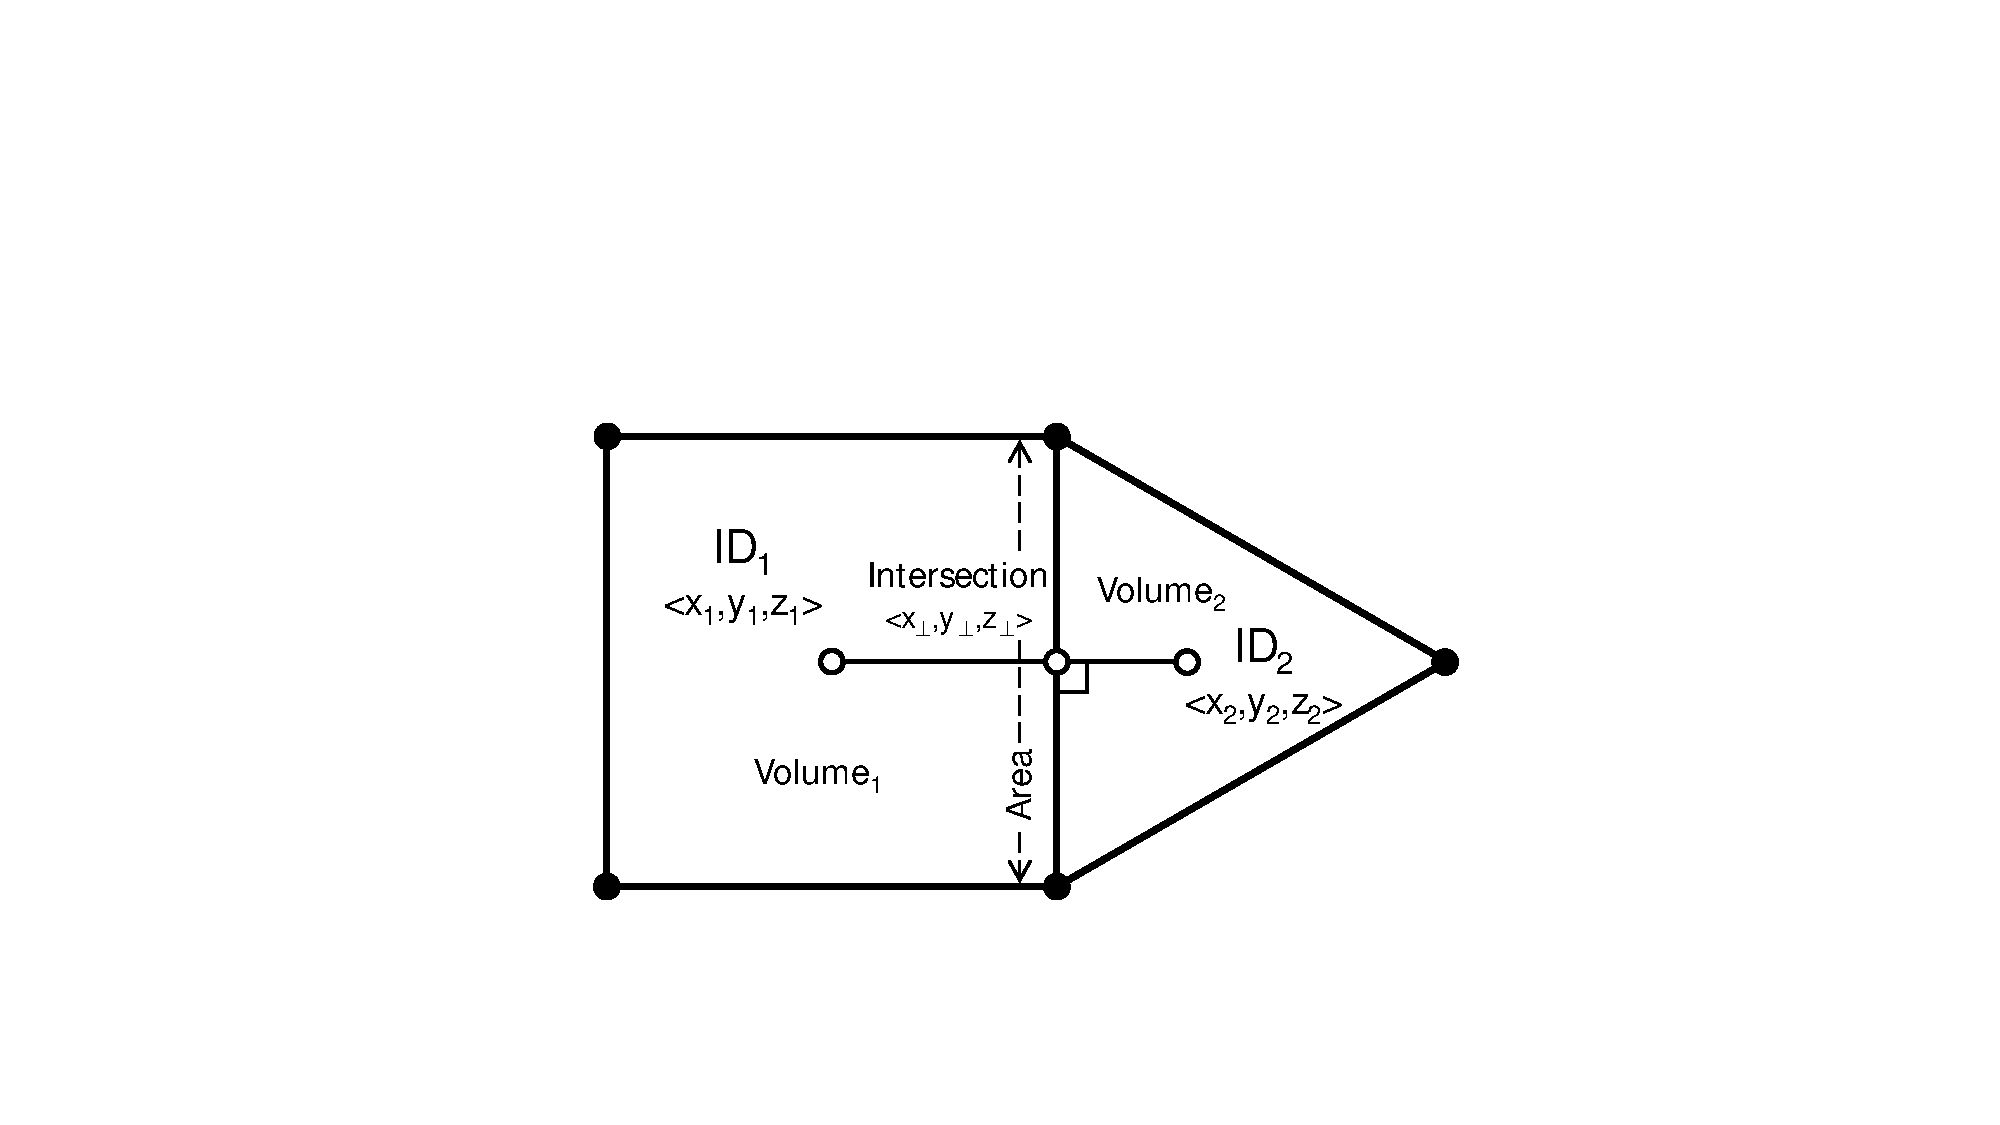
\includegraphics[width=1\linewidth]{./fe_dual}
\end{frame}

\begin{frame}[fragile]\frametitle{UNSTRUCTURED (Distorted)}
\vspace{0.2in}
\centering
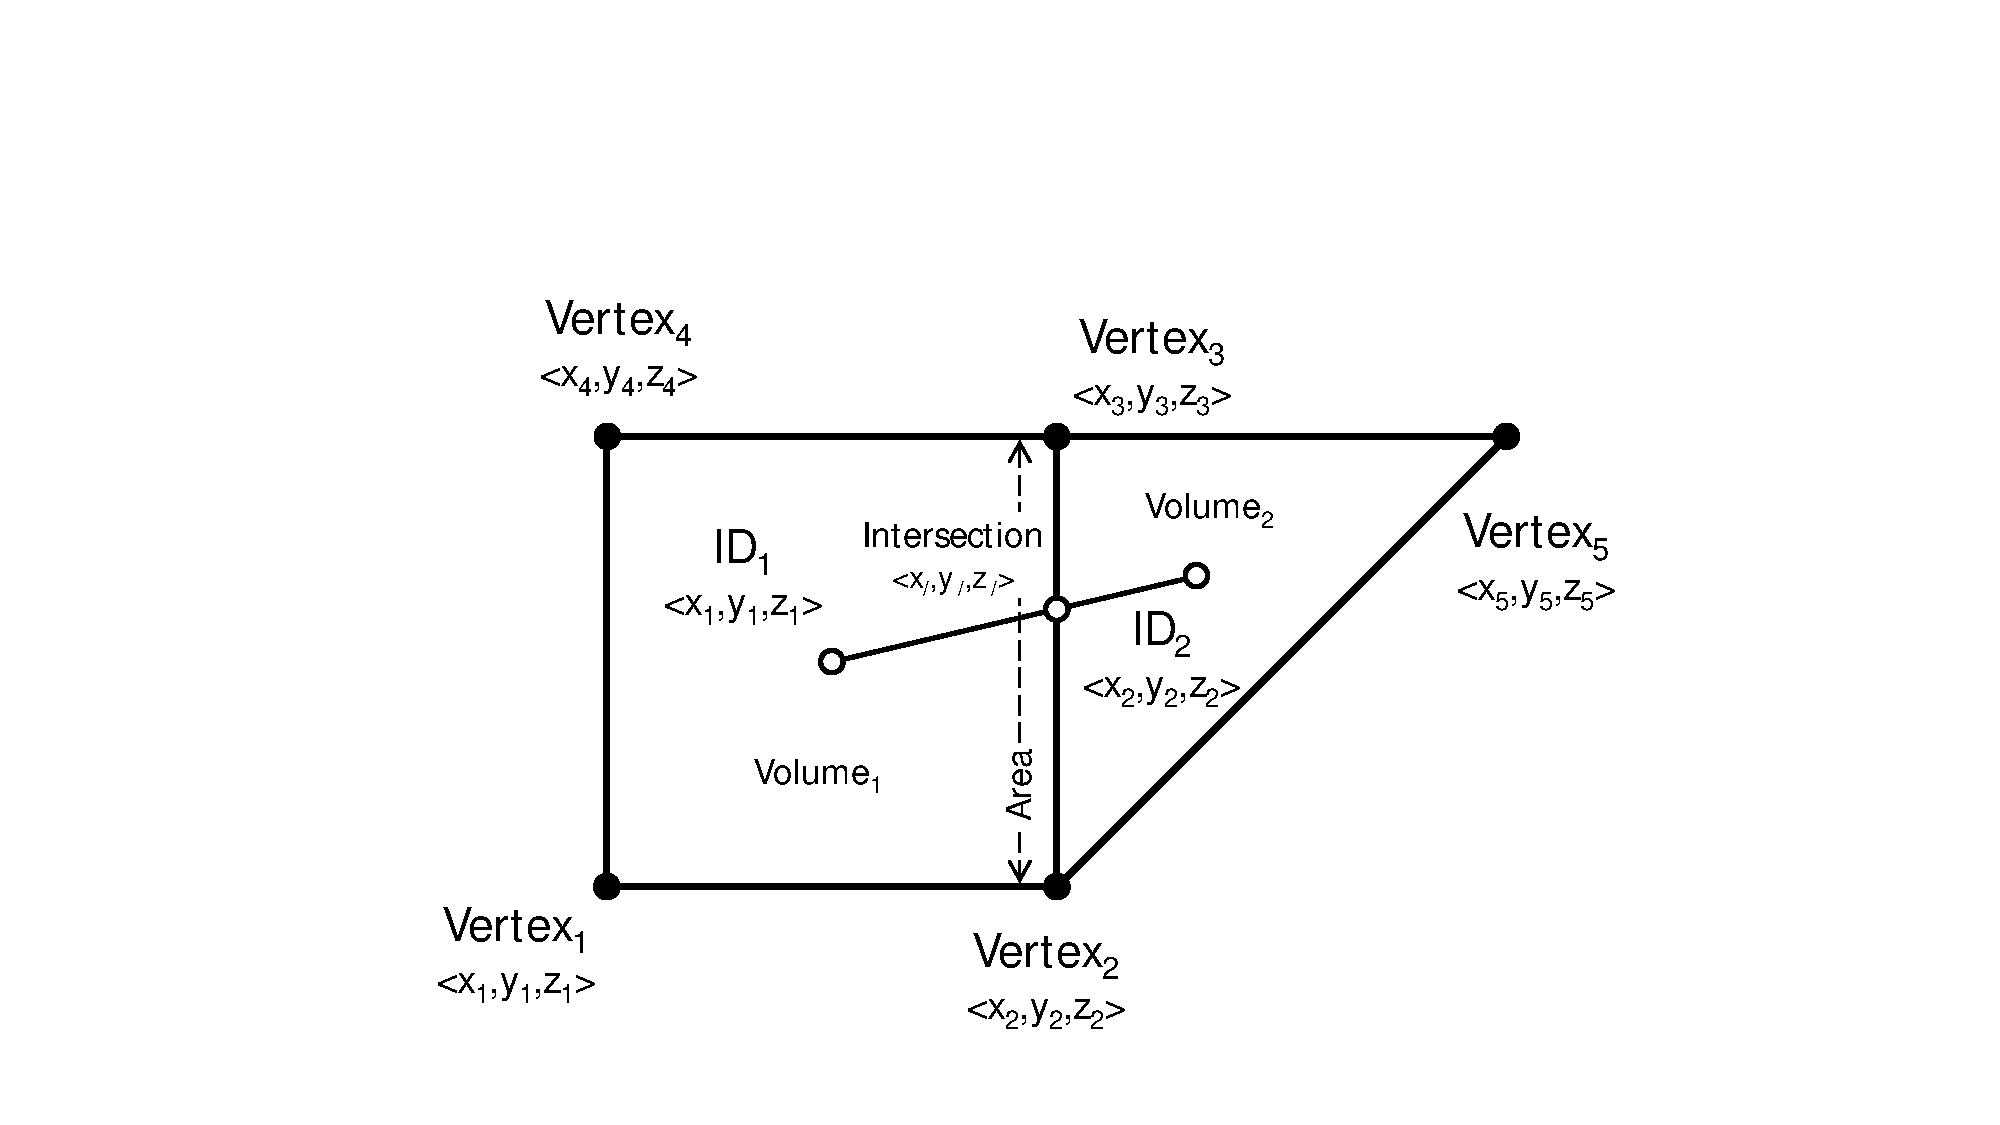
\includegraphics[width=1\linewidth]{./fe_distort_all}
\end{frame}

\begin{frame}[fragile]\frametitle{UNSTRUCTURED (Distorted Connectivity)}
\vspace{0.2in}
\centering
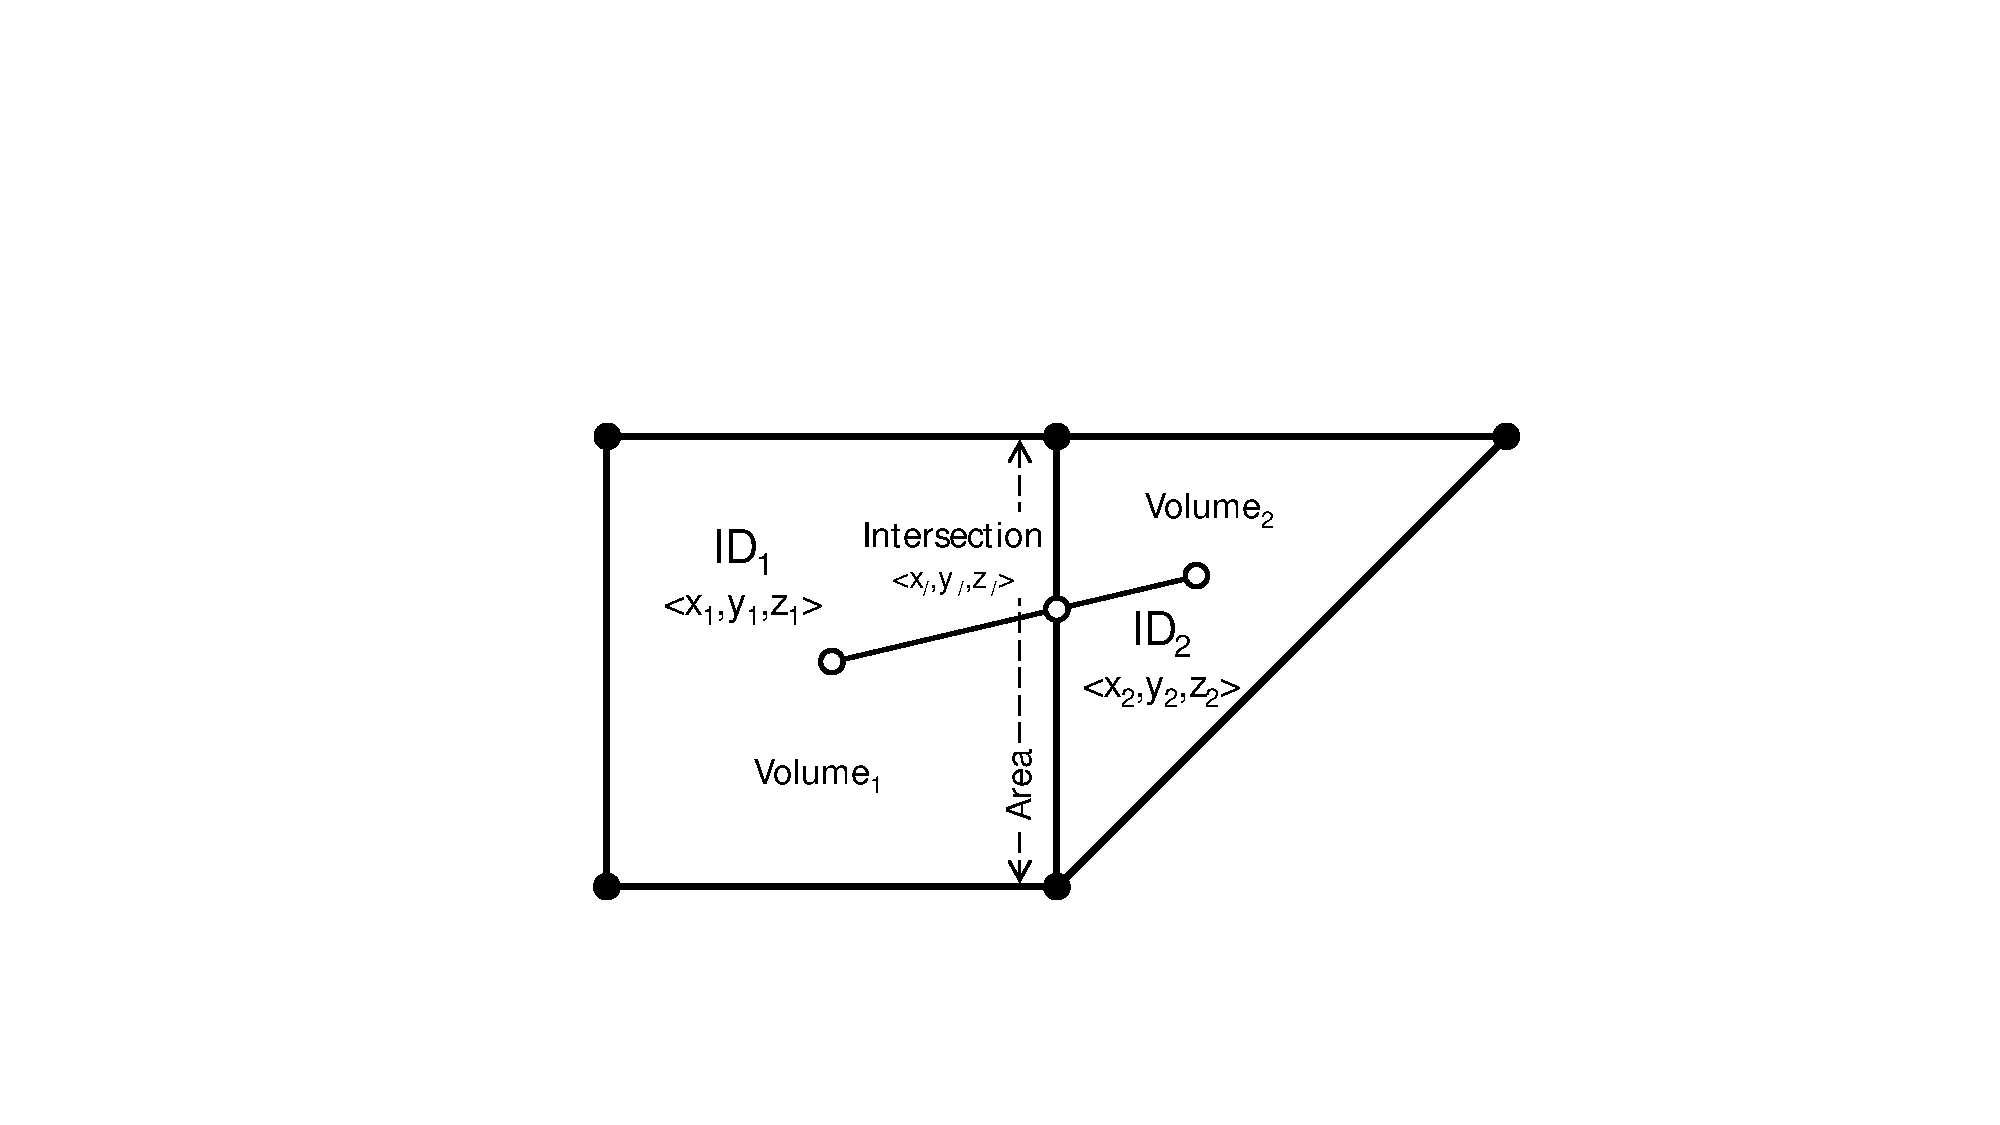
\includegraphics[width=1\linewidth]{./fe_distort_dual}
\end{frame}

\begin{frame}[fragile]\frametitle{UNSTRUCTURED\_EXPLICIT}
\vspace{0.2in}
\centering
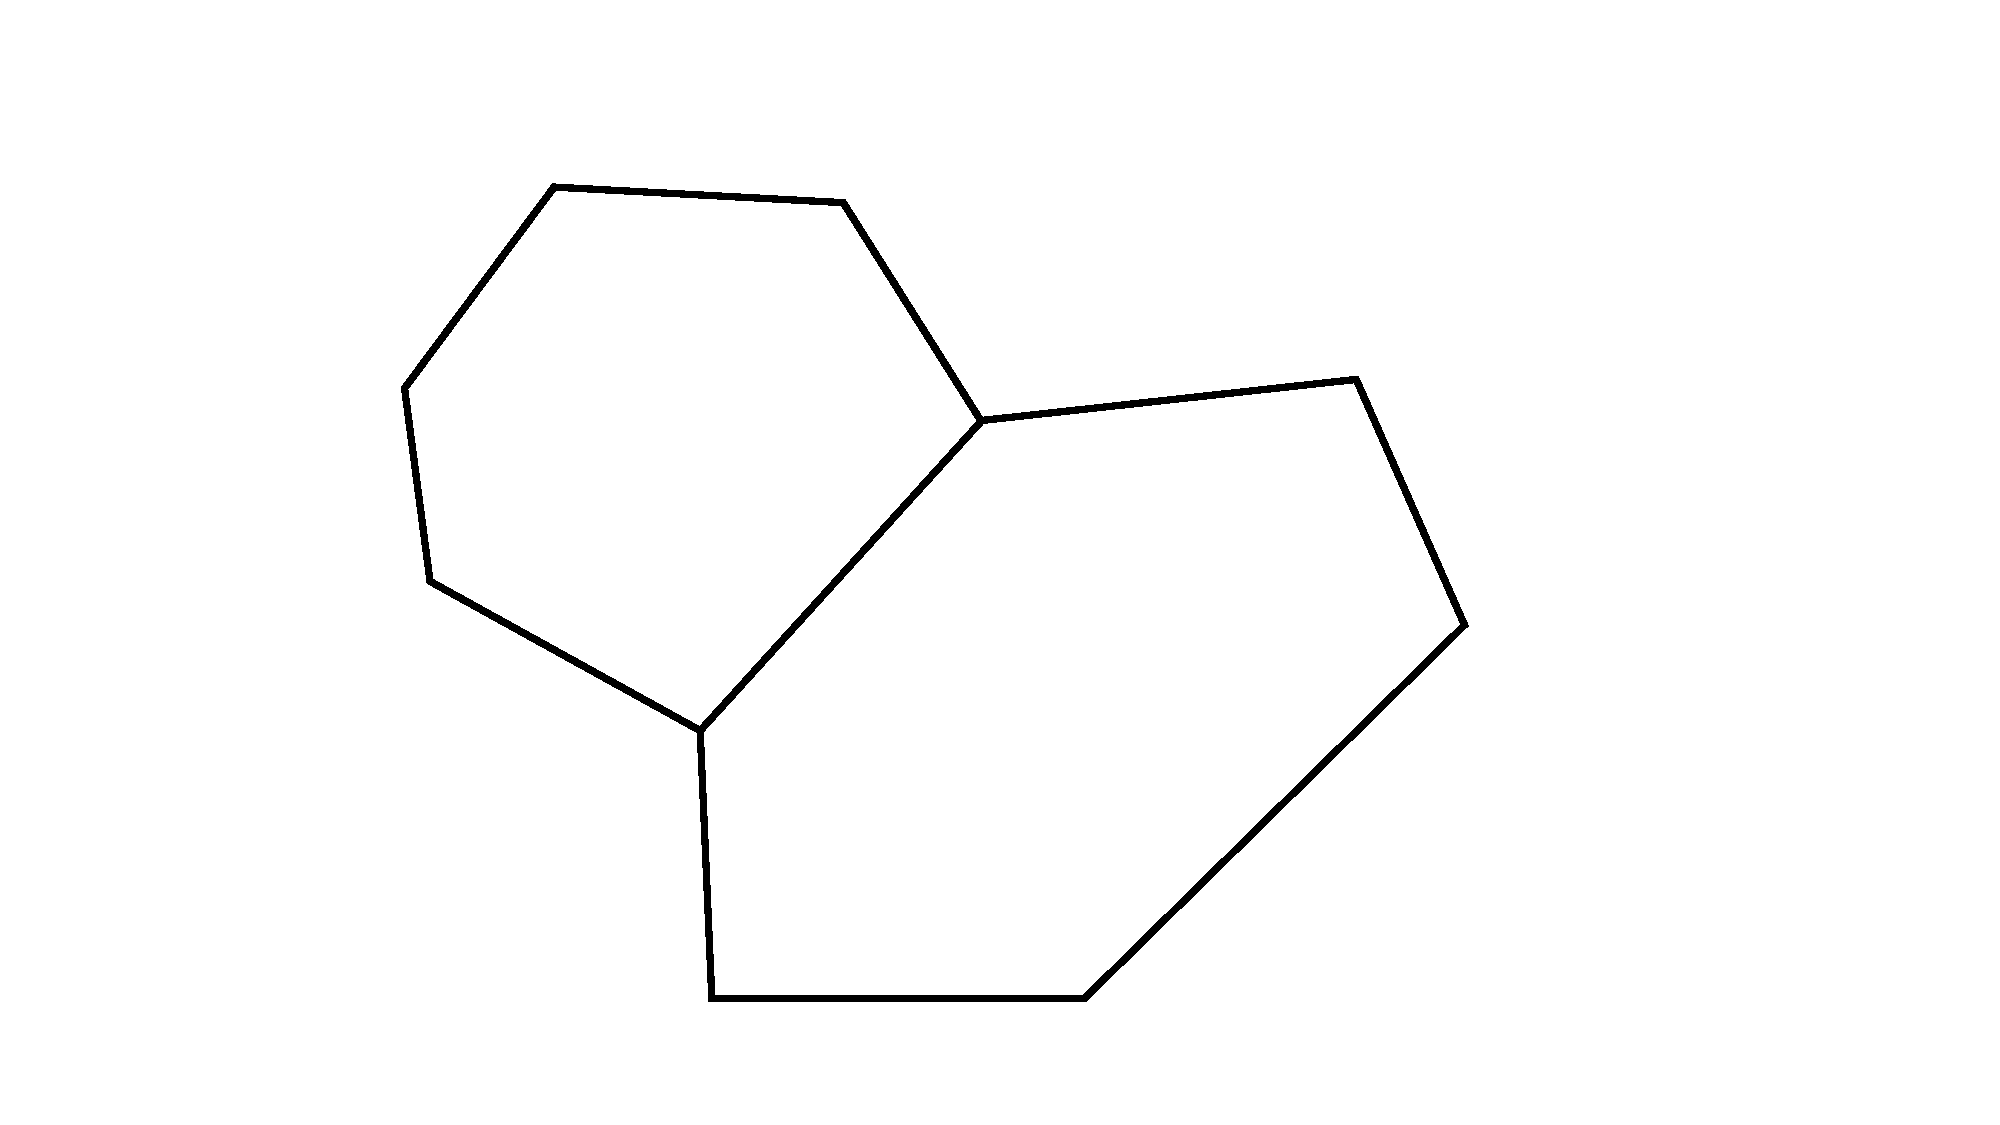
\includegraphics[width=0.9\linewidth]{./voronoi_geom}
\end{frame}

\begin{frame}[fragile]\frametitle{UNSTRUCTURED\_EXPLICIT}
\vspace{0.2in}
\centering
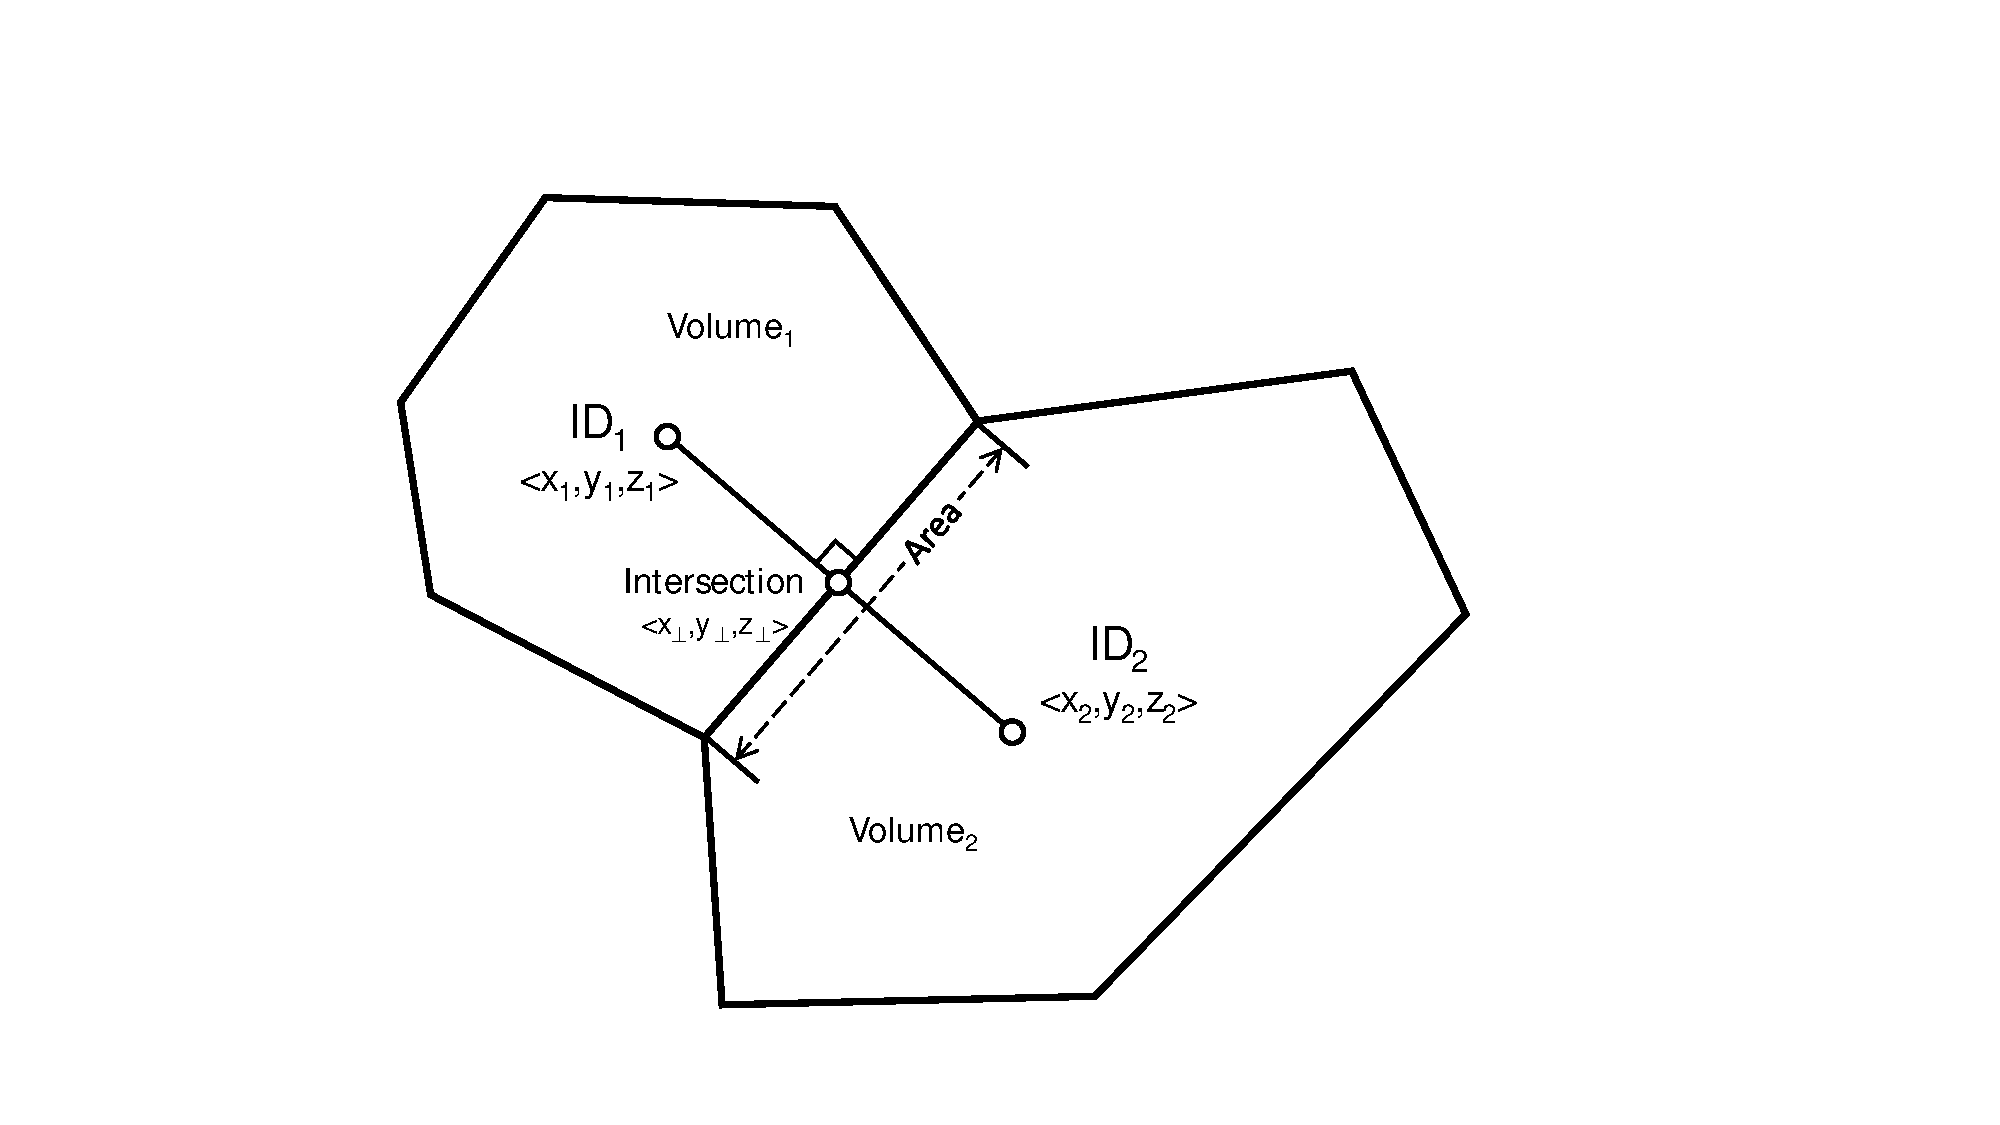
\includegraphics[width=0.9\linewidth]{./voronoi_dual}
\end{frame}

\subsection{Unstructured Grid File Formats}

\begin{frame}[fragile,containsverbatim]\frametitle{UNSTRUCTURED (File Format)}
.ugi file format:
\small
\begin{semiverbatim}
NUM_CELLS NUM_VERTICES
CELL_TYPE VERTEX_1 VERTEX_2 ... VERTEX_N
...
CELL_TYPE VERTEX_1 VERTEX_2 ... VERTEX_N
VERTEX_X_COORDINATE VERTEX_Y_COORDINATE VERTEX_Z_COORDINATE
...
VERTEX_X_COORDINATE VERTEX_Y_COORDINATE VERTEX_Z_COORDINATE
\end{semiverbatim}

Cell Types:
\begin{itemize}
\item T - tetrahedron (4 vertices)
\item P - pyramid (5 vertices)
\item W - wedge (6 vertices)
\item H - hexahedron (8 vertices)
\end{itemize}
\end{frame}

\begin{frame}[fragile,containsverbatim]\frametitle{UNSTRUCTURED (File Format Example)}

\begin{minipage}[t]{0.48\linewidth}
\vspace{0.2in}
.ugi file contents
\begin{semiverbatim}
2 5
Q 1 2 3 4
T 2 5 3
x1 y1 z1
x2 y2 z2
x3 y3 z3
x4 y4 z4
x5 y5 z5
\end{semiverbatim}
\scriptsize
\vspace{0.1in}
\textit{Q is quadrilateral and T is triangle for demonstration only. 2D cells are not supported in PFLOTRAN.}
\end{minipage}
\hfill
\begin{minipage}[t]{0.48\linewidth}
\vspace{0.01in}
\hspace{-.75in}
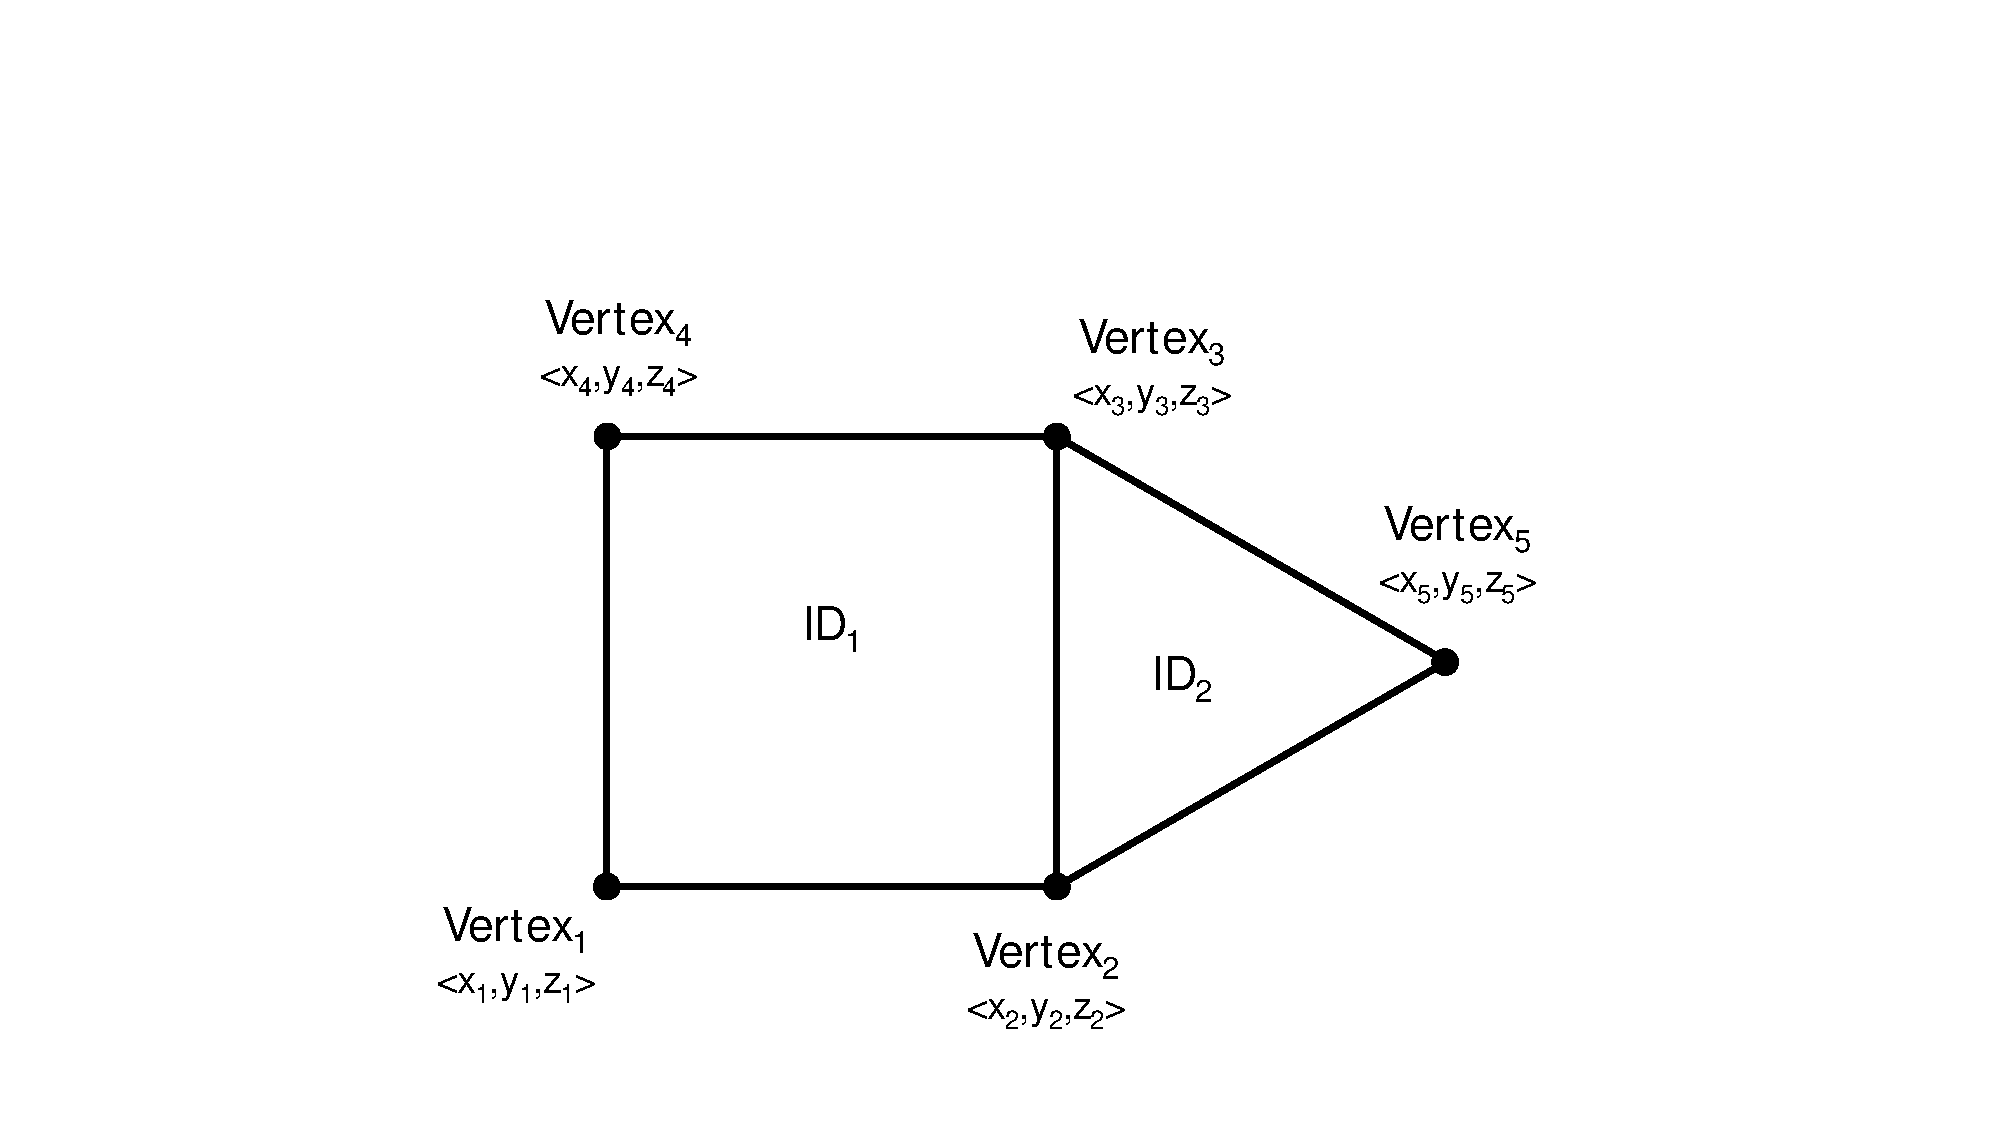
\includegraphics[width=1.5\linewidth]{./fe_raw}
\end{minipage}

\end{frame}

\begin{frame}[fragile,containsverbatim]\frametitle{UNSTRUCTURED\_EXPLICIT (File Format)}
.uge file format:
\begin{semiverbatim}
  CELLS #
  1 X\_coordinate Y\_coordinate Z\_coordinate VOLUME
  ...
  # X\_coordinate Y\_coordinate Z\_coordinate VOLUME
  CONNECTIONS #
  CELL\_a CELL\_b X\_coordinate Y\_coordinate Z\_coordinate AREA
  ...
  CELL\_y CELL\_z X\_coordinate Y\_coordinate Z\_coordinate AREA
\end{semiverbatim}

\end{frame}

\begin{frame}[fragile,containsverbatim]\frametitle{UNSTRUCTURED\_EXPLICIT (File Format Example)}

\begin{minipage}[t]{0.48\linewidth}
\vspace{0.4in}
.uge file contents
\begin{semiverbatim}
CELLS 2
1 x1 y1 z1 Volume1
2 x2 y2 z2 Volume2
CONNECTIONS 1
1 2 x| y| z| Area
\end{semiverbatim}
\end{minipage}
\hfill
\begin{minipage}[t]{0.48\linewidth}
\vspace{0.01in}
\hspace{-.5in}
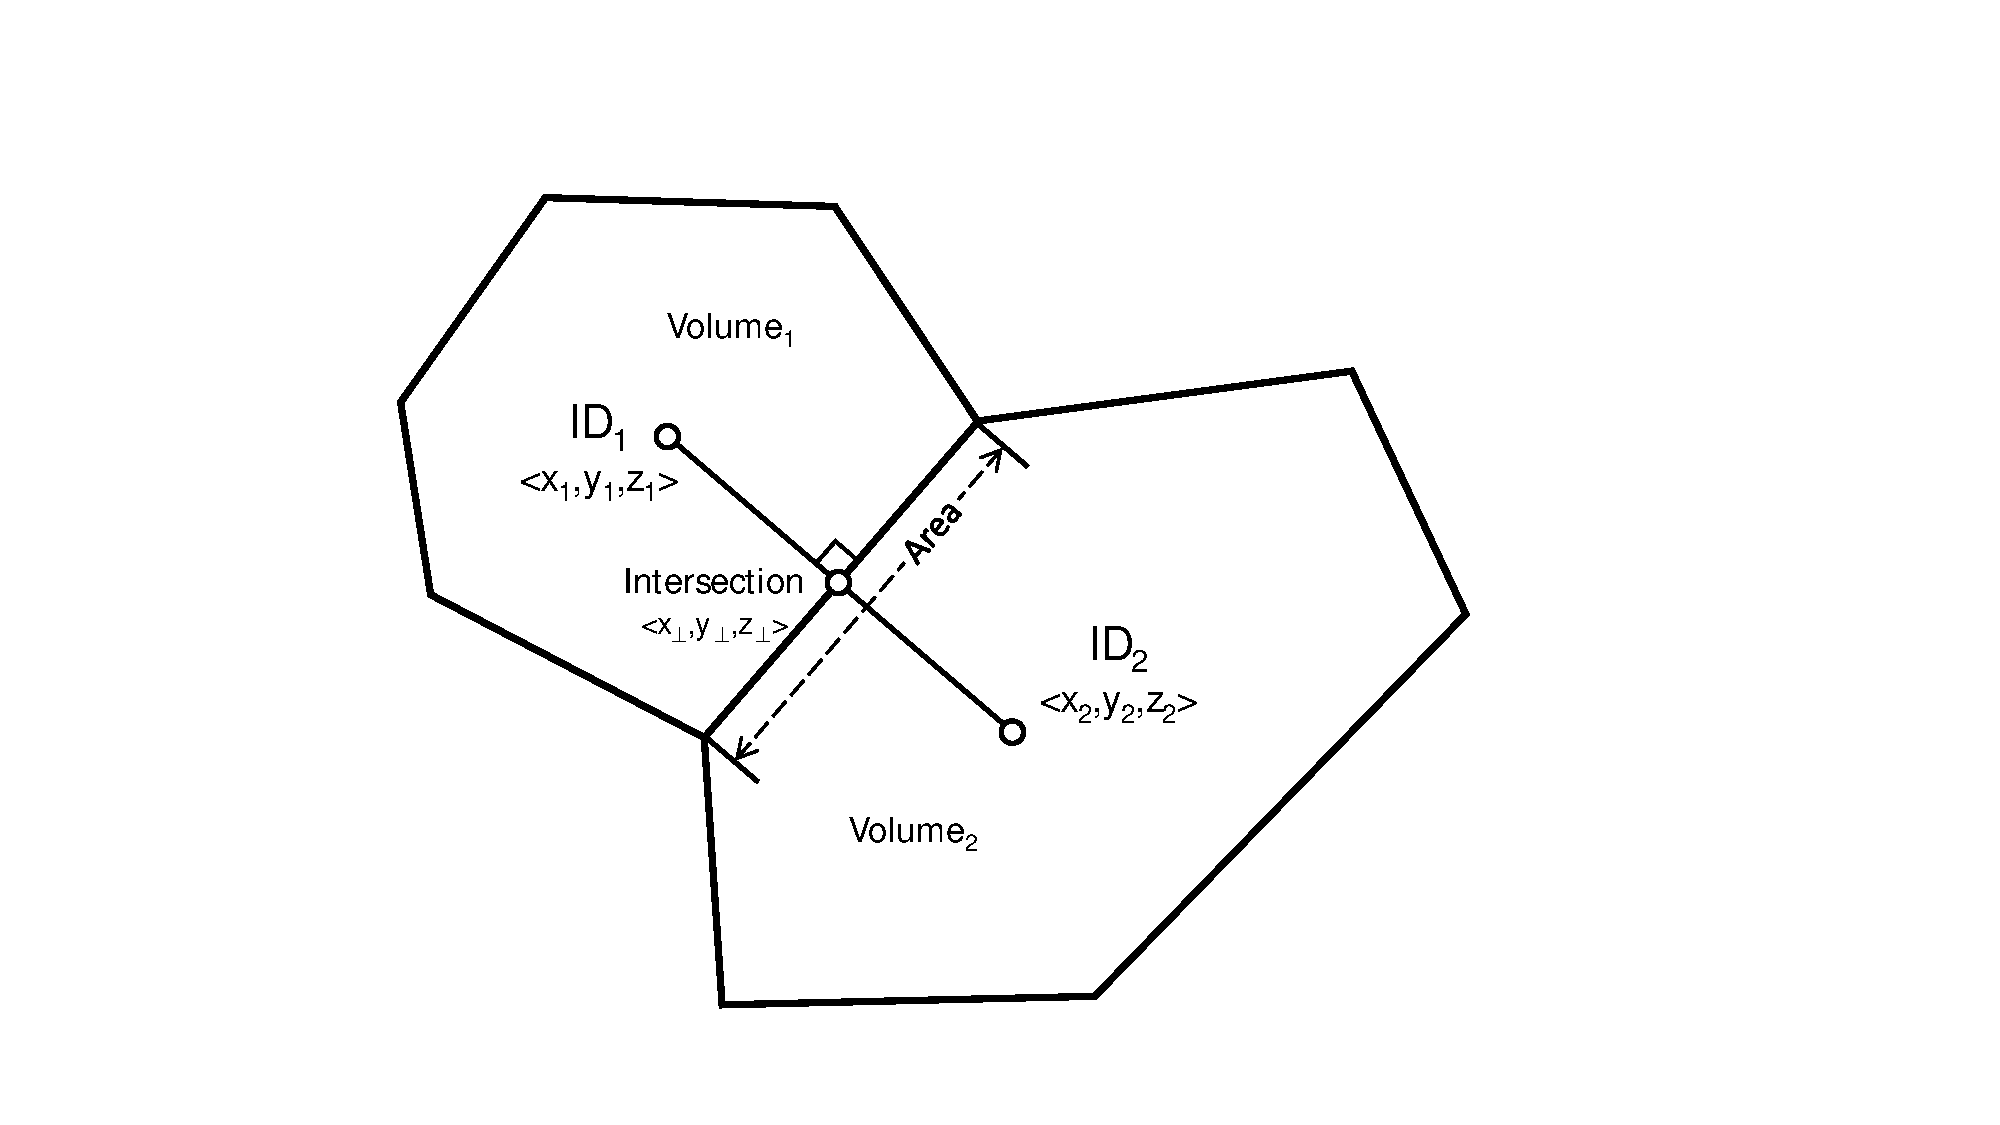
\includegraphics[width=1.3\linewidth]{./voronoi_dual}
\end{minipage}

\end{frame}

\subsection{Unstructured Grid Examples}

\begin{frame}[fragile,containsverbatim]\frametitle{mixed.ugi file contents}

\begin{minipage}[t]{0.48\linewidth}
  \begin{semiverbatim}
15 24
P 4 5 6 2 1
T 4 3 5 1
W 2 7 6 4 9 5
W 8 7 2 10 9 4
W 10 9 4 21 14 11
H 19 9 5 12 17 7 6 16
T 5 13 14 15
T 5 14 9 15
P 5 9 19 12 15
...
P 22 23 14 13 15
5.000000e+00 5.000000e+00 5.000000e+00
5.000000e+00 2.500000e+00 5.000000e+00
...
0.000000e+00 0.000000e+00 0.000000e+00
  \end{semiverbatim}
\end{minipage}
\hfill
\begin{minipage}[t]{0.48\linewidth}
  \vspace{-0.5in}
  \hspace{-.5in}
  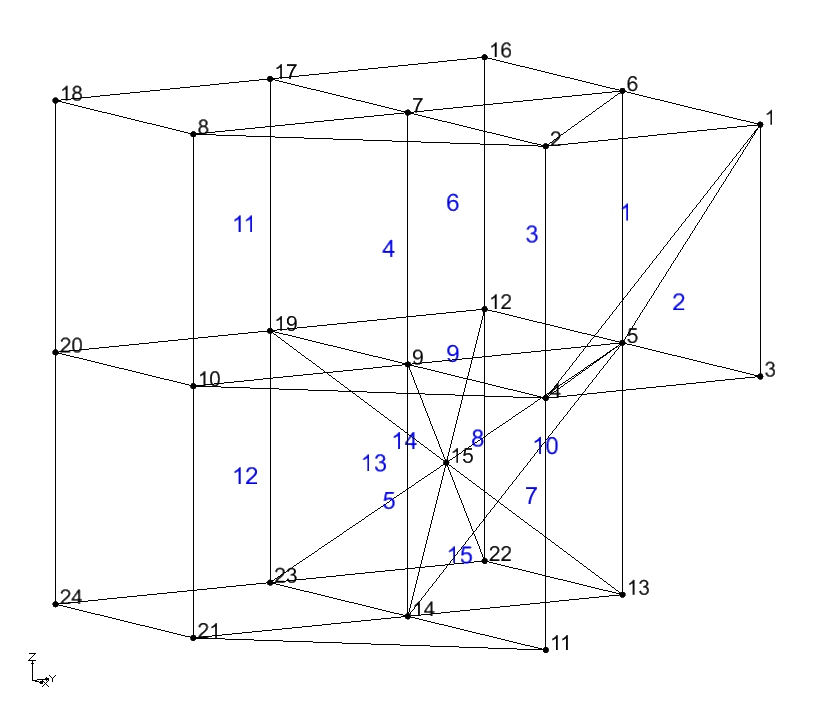
\includegraphics[width=1.4\linewidth]{./mixed}
\end{minipage}

\end{frame}

\begin{frame}[fragile,containsverbatim]\frametitle{mixed.h5 file contents}

\begin{minipage}[t]{0.48\linewidth}
\vspace{-0.1in}
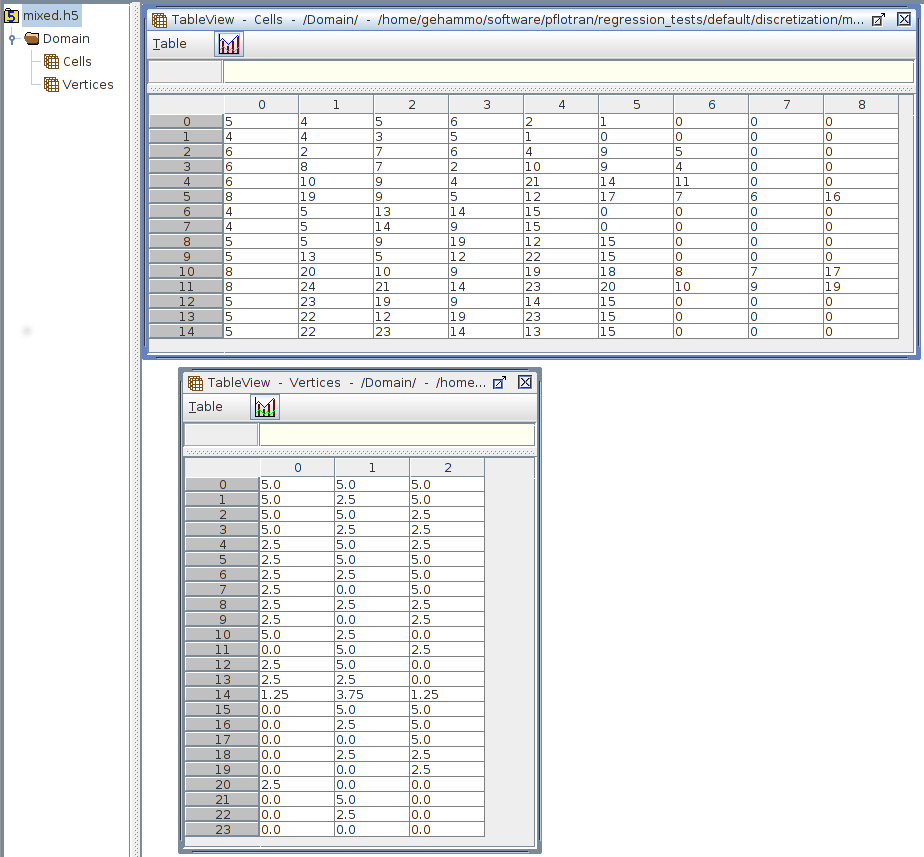
\includegraphics[width=1.8\linewidth]{./mixed_h5.png}
\end{minipage}
\hfill
\begin{minipage}[t]{0.48\linewidth}
  \vspace{1.4in}
  \hspace{.1in}
  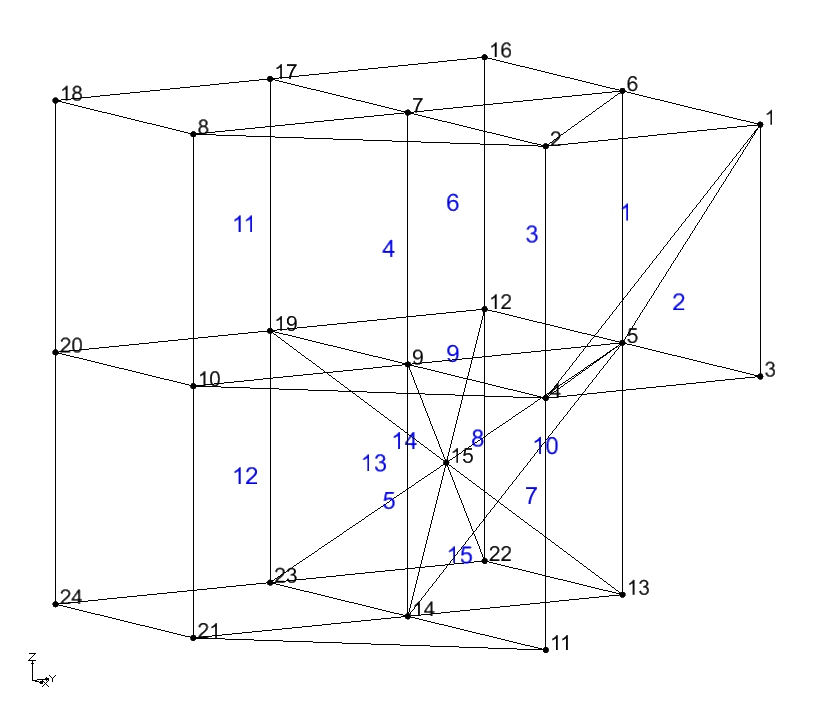
\includegraphics[width=1.\linewidth]{./mixed}
\end{minipage}

\end{frame}

\begin{frame}[fragile,containsverbatim]\frametitle{mixed.uge file contents}

\begin{minipage}[t]{0.48\linewidth}
  \small
  \begin{semiverbatim}
CELLS 15
1 4.0625 4.0625 4.0625 5.20833
2 4.375 4.375 3.125 2.60417
3 3.3333 3.3333 3.75 7.8125
4 3.3333 1.6667 3.75 7.8125
5 3.3333 1.6667 1.25 7.8125
6 1.25 3.75 3.75 15.625
...
15 1.25 3.75 0.3125 2.60417
CONNECTIONS 24
1 2 4.16667 4.16667 3.3333 6.25
1 3 3.75 3.75 3.75 8.8388
3 4 3.75 2.5 3.75 6.25
3 6 2.5 3.75 3.75 6.25
4 5 3.3333 1.6667 2.5 3.125
4 11 2.5 1.25 3.75 6.25
5 12 2.5 1.25 1.25 6.25
6 9 1.25 3.75 2.5 6.25
...
14 15 0.41667 3.75 0.41667 2.2097
  \end{semiverbatim}
\end{minipage}
\hfill
\begin{minipage}[t]{0.48\linewidth}
  \vspace{0.1in}
  \hspace{.0in}
  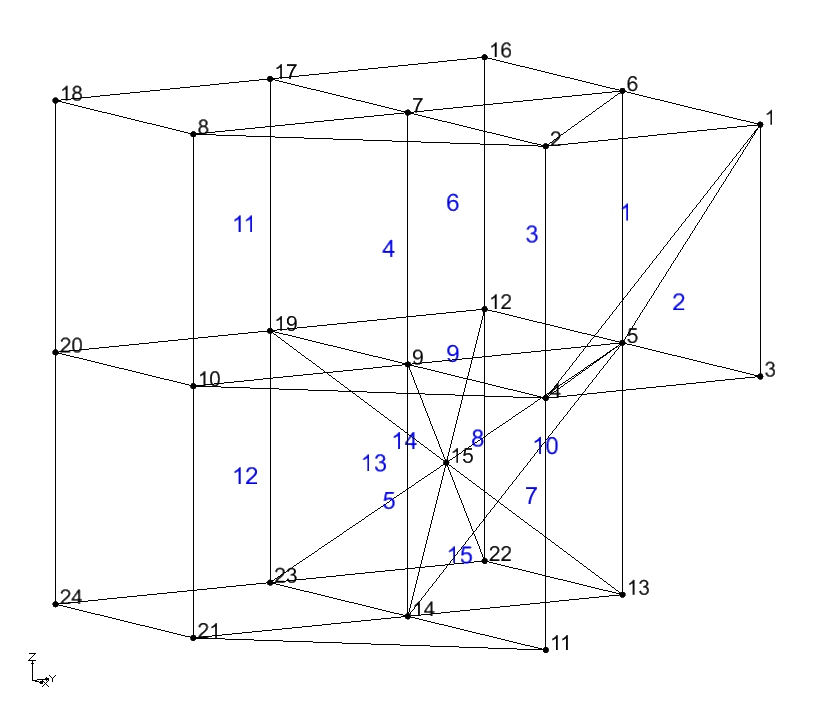
\includegraphics[width=1.2\linewidth]{./mixed}
\end{minipage}

\end{frame}

\end{document}
